%% 
%% Copyright 2007-2020 Elsevier Ltd
%% 
%% This file is part of the 'Elsarticle Bundle'.
%% ---------------------------------------------
%% 
%% It may be distributed under the conditions of the LaTeX Project Public
%% License, either version 1.2 of this license or (at your option) any
%% later version.  The latest version of this license is in
%%    http://www.latex-project.org/lppl.txt
%% and version 1.2 or later is part of all distributions of LaTeX
%% version 1999/12/01 or later.
%% 
%% The list of all files belonging to the 'Elsarticle Bundle' is
%% given in the file `manifest.txt'.
%% 

%% Template article for Elsevier's document class `elsarticle'
%% with numbered style bibliographic references
%% SP 2008/03/01
%%
%% 
%%
%% $Id: elsarticle-template-num.tex 190 2020-11-23 11:12:32Z rishi $
%%
%%
\documentclass[preprint,12pt]{elsarticle}

%% Use the option review to obtain double line spacing
%% \documentclass[authoryear,preprint,review,12pt]{elsarticle}

%% Use the options 1p,twocolumn; 3p; 3p,twocolumn; 5p; or 5p,twocolumn
%% for a journal layout:
%% \documentclass[final,1p,times]{elsarticle}
%% \documentclass[final,1p,times,twocolumn]{elsarticle}
%% \documentclass[final,3p,times]{elsarticle}
%% \documentclass[final,3p,times,twocolumn]{elsarticle}
%% \documentclass[final,5p,times]{elsarticle}
%% \documentclass[final,5p,times,twocolumn]{elsarticle}

%% For including figures, graphicx.sty has been loaded in
%% elsarticle.cls. If you prefer to use the old commands
%% please give \usepackage{epsfig}

%% The amssymb package provides various useful mathematical symbols
\usepackage{amssymb}
%% The amsthm package provides extended theorem environments
%% \usepackage{amsthm}

%% The lineno packages adds line numbers. Start line numbering with
%% \begin{linenumbers}, end it with \end{linenumbers}. Or switch it on
%% for the whole article with \linenumbers.
%% \usepackage{lineno}

\journal{JuliaCon Proceedings}

\begin{document}
\sloppy

\begin{frontmatter}

%% Title, authors and addresses

%% use the tnoteref command within \title for footnotes;
%% use the tnotetext command for theassociated footnote;
%% use the fnref command within \author or \address for footnotes;
%% use the fntext command for theassociated footnote;
%% use the corref command within \author for corresponding author footnotes;
%% use the cortext command for theassociated footnote;
%% use the ead command for the email address,
%% and the form \ead[url] for the home page:
%% \title{Title\tnoteref{label1}}
%% \tnotetext[label1]{}
%% \author{Name\corref{cor1}\fnref{label2}}
%% \ead{email address}
%% \ead[url]{home page}
%% \fntext[label2]{}
%% \cortext[cor1]{}
%% \affiliation{organization={},
%%             addressline={},
%%             city={},
%%             postcode={},
%%             state={},
%%             country={}}
%% \fntext[label3]{}
\title{MedVoxelHD: Improved CUDA-accelerated morphological Hausdorff distances in medical image analysis}

%% use optional labels to link authors explicitly to addresses:
%% \author[label1,label2]{}
%% \affiliation[label1]{organization={},
%%             addressline={},
%%             city={},
%%             postcode={},
%%             state={},
%%             country={}}
\ead{jakub.mitura14@gmail.com}
%%  
%% \affiliation[label2]{organization={},
%%             addressline={},
%%             city={},
%%             postcode={},
%%             state={},
%%             country={}}

\author[inst1,inst2]{Jakub Mitura}



\author[inst2]{Beata E. Chrapko}

\affiliation[inst1]{organization={National Information Processing Institute},%Department and Organization
            addressline={al. Niepodległości 188 B}, 
            city={Warsaw},
            postcode={00-608}, 
            state={woj. Mazowieckie},
            country={Poland}}


\affiliation[inst2]{organization={Medical University of Lublin},%Department and Organization
            addressline={Al. Racławickie 1}, 
            city={Lublin},
            postcode={20-059}, 
            state={woj. Lubelskie},
            country={Poland}}

\begin{abstract}
%% Text of abstract
Medical image segmentation is a rapidly developing field of computer vision. This area of research requires knowledge in radiologic imaging, mathematics, and computer science. Multiple software packaged have been developed to  assist researchers in the field. However, due to the rapidly changing scientific environment, some tools are longer  effective for some users. This is the case of Julia language users that require support for the interactive programming development style that is not popular among traditional software tools. Other characteristic of modern programming for 3 dimensional medical imaging data is GPU acceleration which can give outstanding improvement of algorithms performance in case of working on object that can be represented as big arrays like those present in 3D medical imaging. Hence in this work author presents sets of new Julia language software tools that are designed to fulfill emerging needs. Those tools encompass GPU accelerated medical image viewer with annotation possibility that is characterized by very convenient programming interface. CUDA accelerated Medical segmentation metrics tool that supply state of the art implementations of algorithms required for quantification of similarity between algorithm output and gold standard. Lastly set of utility tools connecting those two mentioned packages with HDF5 file system.
\end{abstract}

\begin{keyword}
%% keywords here, in the form: keyword \sep keyword
CUDA \sep computer tomography \sep medical image segmentation
%% PACS codes here, in the form: \PACS code \sep code

\end{keyword}

\end{frontmatter}

%% \linenumbers

%% main text

\section{Introduction}
One of the fields of computer vision that has potential immediate influence on society well being is automatizing of diagnosis based on medical imaging. In order to recognize and label both pathological and physiological structures one can use multiple algorithms that are known under the label of medical image segmentation algorithms . As in any other field of computer vision one can define supervised, semi supervised and non supervised methods. Another way of dividing those methods is into automatic and semiautomatic, where in latter some  user input is required.

Typical workflow includes:
\begin{enumerate}
  \item visual inspection of  the data, and exploration of metadata.
  \item feature engineering in order to represent data in a way that would be most effective in chosen model.
  \item choosing model considering possible assumptions that could be encoded in a model as inductive bias.
  \item choosing segmentation metric and cost function.
  \item after evaluation and debugging one need to reconsider design choices in order to improve model performance.
  \item reiterate until the model performance will be satisfactory.
\end{enumerate}

For all of the steps above multiple software tools are already widely available.
However in order to implement any model in a robust and efficient manner one need to use appropriate tools for given domain. This includes considerations on: size of single image file, performance constraints, interoperability of the required tools, language of the package interface and many others.

For 3D medical image segmentation typical problem is related to size of the images which can frequently reach multiple gigabytes per patient. Such size dictates requirement of parallelization in order to achieve acceptable execution times. Currently most effective parallelization in case of medical imaging can be achieved using GPU architectures.  Hence according to the author in case of tools used for medical segmentation metrics possibility of GPU acceleration is highly desirable. Luckily such tools are available for example in MONAI \cite{MONAI} or tensorflow \cite{tensorflow}. However most of the tools available has interface written in python programming language. This can be considered as advantage because it makes collaboration between data scientists easier, as python is most popular data science language, and is considered as easy to use. Yet it also leads to some Python specific issues. Most important is relatively low performance. Popular python libraries usually solve the problem by writing main code in high performance language like C++ and supplying python interface to it. However apart from additional work needed to write and maintain such libraries it leads to big problem with interoperability of such python packages. This is know as two language problem and one of the best solutions to it is Julia programming language \cite{Julia}. Additionaly Julia language ecosystem contain multiple packages supporting varius aspects of GPU programming among others CUDA.jl \cite{besard2019prototyping} and ParallelStencil.jl \cite{ParallelStencil}.

\section{Visual inspection}

\begin{figure}[t!]
	\centering
	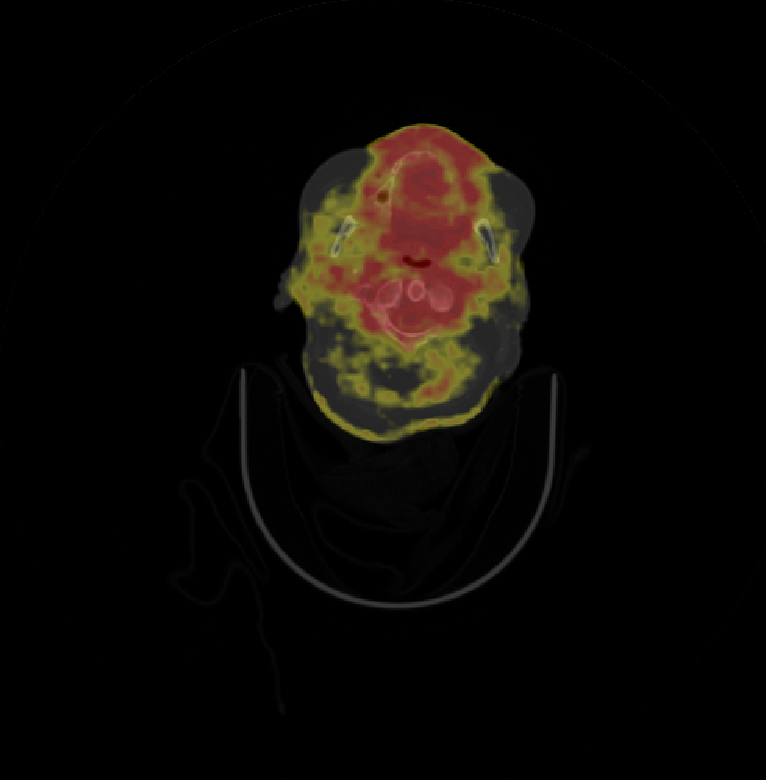
\includegraphics[width=0.95\textwidth]{PETCTCORONAL.png}
	\caption{transverse Display FDG PET/CT}
	\label{fig:PETCTCORONAL}
	\centering
\end{figure}

Visual inspection in case of 3D data requires special software. Although multiple high quality applications created for viewing and annotating are available most of them require special configuration and are not always convenient to use during rapid development phase. In Julia programming language typical workflow includes constant experimenting using interactive environment Read–eval–print loop (REPL) which increase development efficiency. However currently available 3D visualization tools are not well suited for such workflow. In order to address this issue author had developed new  3D visualization and annotation tool MedEye3d \cite{Mitura2021} which is characterized by high performance, low memory consumption, and interface that is created to be easily accessible from REPL command line or from keyboard shortcuts. Additionally because of the intended usage pattern no typical graphical user interface elements (like buttons etc.) are added. This decrease the surface on the screen occupied by the application and makes it easier to use it as a separate window next to chosen Julia Integrated development environment (IDE). Despite purposeful simplicity all crucial functionalities required for displaying 3D medical imaging are easily available via keyboard shortcuts. Also in case of development of semiautomatic algorithms annotations on the image are easy to perform and results are immediately available in the Julia REPL for further processing. Example display can be seen in figure \ref{fig:PETCTCORONAL}.

\section{Problem Statement and Research Objectives}
Although Julia programming language is characterized by plethora of excellent scientific software packages to the best knowledge of the author lacks some of the necessary tools in the area of 3D medical segmentation .Most problematic seem to be lack of efficient visualization and evaluation tools. The goal of this work is to provide scientific community with those missing software solutions, and popularize through it the study on the 3D medical segmentation in Julia language community.


\section{Evaluation metrics}

The choice of evaluation metric is dictated mainly by two considerations. First is that the chosen metric quantifies similarity between some gold standard and output of the algorithm. In order to be able to asses it one need to have some measure of domain knowledge related to the data on which the algorithm will be run.  The other requirement is that chosen metric function will have properties required for optimization. In most cases it means that one can define the gradient of the metric, so it can be used for example in back propagation of the neural network. The latter requirement leads in some cases to modifications of the metric function itself. The metric that is subjected to optimization algorithm is called cost function and by convention small values should represent big similarity between compared data.  However arguably first consideration is more important from algorithm design perspective, as researcher needs to be sure that reduction of the cost function value is truly related to increasing similarity between measured entities in a meaningful way. Hence the cost functions traditionally defined for standard images frequently can not be readily used in the task of measuring the similarity between gold standard and algorithm output for the medical image segmentation. Problem is particularly evident in case of 3 dimensional data.

In the field of medical segmentation probably most influential works describing segmentation metrics were those published by Renard et al \cite{Nature} and by Taha et al \cite{TahaMainSegm}. Those works stressed that optimal metric may be different depending on the problem. So for example in multiple cases there is big interclass discrepancy in relation to its representation in data, because of it one of the most commonly used segmentation metric is Dice metric. In work of Taha et al \cite{TahaMainSegm} multiple algorithms including before mentioned Dice metric are implemented using confusion matrix ( which includes amount of true positive, false positive, true negative and false negative entries). This group of algorithms open new easily available opportunities to use multiple metrics at once without significant performance penalty, and validate using some other criteria (for example visual inspection). However frequently not only amount of voxels that are correctly or incorrectly labeled is important but also their spatial distribution. In this case one should consider distance metric like mahalanobis or hausdorff distance.  However algorithms that take distance in consideration are typically far more computationally intensive.

Currently in the subfield of machine learning concentrated around medical imaging segmentation metrics there are two main frameworks Pymia \cite{Pymia} and Monai \cite{MONAI}, in both cases user interface is written in Python. Monai \cite{MONAI} implements multiple  highly optimized metrics that are particularly prevalent in case of neural networks with available Compute Unified Device Architecture (CUDA) acceleration , yet lacks most of those described in \cite{TahaMainSegm}. It is also based on PyTorch \cite{pytorch}. Pymia \cite{Pymia} implements all of the algorithms described in  \cite{TahaMainSegm}, is framework independent , but lacks GPU acceleration. GPU acceleration can drastically increase performance in case of large data objects - and such case is very common in modern medical imaging. 


\section{Data management}
Medical imagiing data in clinical setting is usually stored in Digital imaging and communications in medicine (DICOM)  \cite{dicom}. Additionaly DICOM format apart from storing data representing given variable in each voxel of the study, is able to hold rich metadata like patient name, age, details about acquisition technique etc.  However the format was primarily designed for optimizing display and storage of the data and not its processing, hence operations like partial loading or queries of the data lacks efficiency.

Hierarchical Data Format HDF5 \cite{hdf5} is the format that is originating from high performance computing ecosystem. Currently it is recognized as efficient and convenient data format for  storing and processing medical imaging data \cite{hdf5Medical}. Apart from high performance this format is characterized by ability to save and process multidimensional data, and is optimized for large multidimensional arrays. This characteristic is uncommon as most traditional data formats are optimized for tabular data, and stores image data usually in a form of a binary object data type (BLOB), with a limitation that no queries can be performed for data in a BLOB. HDF5 format contrary to BLOB make query and partial loading of stored multidimensional arrays, similarly to other popular data formats it has programming API in multiple widely used languages like Python, C++ and Julia.

HDF5 data format  seem to be optimal for processing 3 dimensional medical imaging as it has perfect support for multidimensional data, is supporting saving metadata of those arrays like DICOM format, and has good query performance and convenient programming interfaces like traditional database formats . Additionally important and quite unique feature is possibility of direct data loading from persistent storage to GPU global memory without intermediate storage in Central Processing Unit (CPU) Random access memory (RAM) \cite{hdf5GPU} . However this last feature will not be used in the presented work for sake of simplicity.

\subsection{Experiments}
\subsubsection{Evaluation metrics}
All experiments were conducted on Windows PC (Intel Core I9 10th gen., GeforceRTX 3080), and Data from CT-ORG \cite{CTORG} dataset, on image of size ($512 \times 512 \times 826$). Time needed to calculate metrics was estimated in case of Julia code using BenchamrkTools.jl \cite{BenchmarkTools}. For testing python libraries internal python module timeit was utilized. Results of experiments mentioned above are summarized in Figure \ref{fig:bk}. In all cases data was already in RAM memory for CPU computation or in GPU memory for CUDA computations - hence memory transfer times were not included.

\begin{figure}[h!]
	\centering
	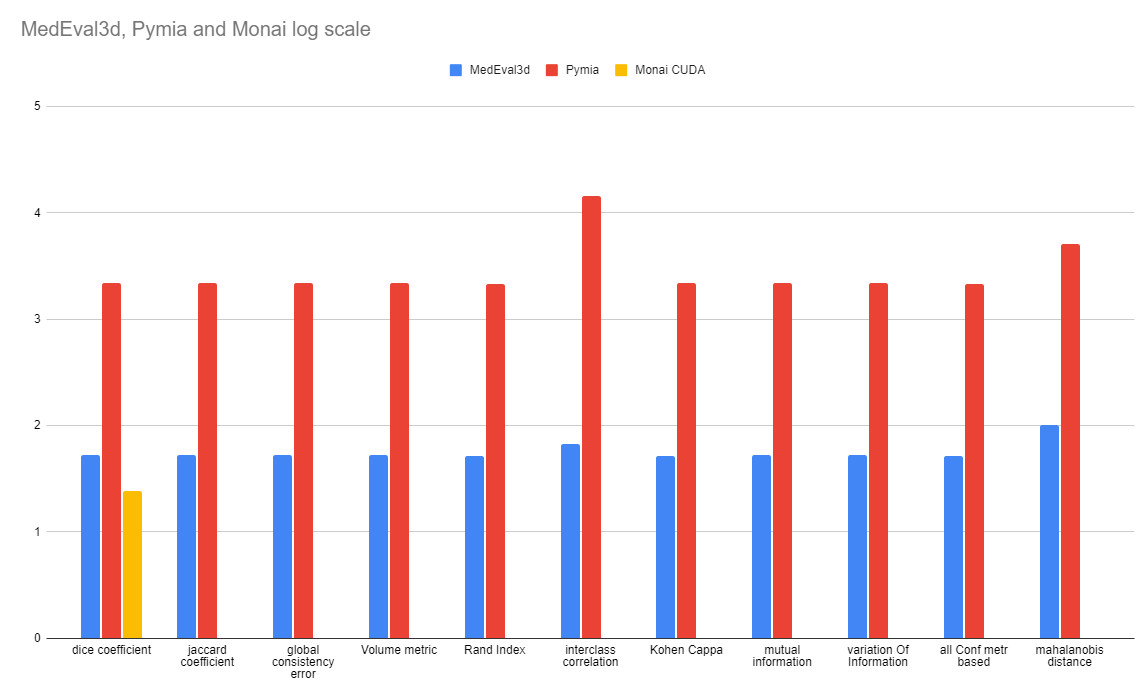
\includegraphics[width=\columnwidth]{bk.png}
	\caption{Comparison of median times needed to calculate given metrics in log scale, for Monai only CUDA accelerated algorithm was taken into account. Dimensionality of data was ($ 512x512x826 $)  }
	\label{fig:bk}
\end{figure}

\subsubsection{Visualization}

In order to measure actual time to  render the GPU synchronization was performed using OpenGl  glFinish() function.
Cross Section plane translation is defined as changing the single coordinate which defines the plane in the chosen cross section. Time needed to accomplish it is measured in milliseconds between rendering commands using BenchamrkTools.jl \cite{BenchmarkTools}. 

Response to mouse left click time was measured as a difference of time reported in the callback registered to GLFW window and end of the execution of a rendering command designed to render the visible change on the chosen texture.

\begin{figure}[t!]
	\centering
	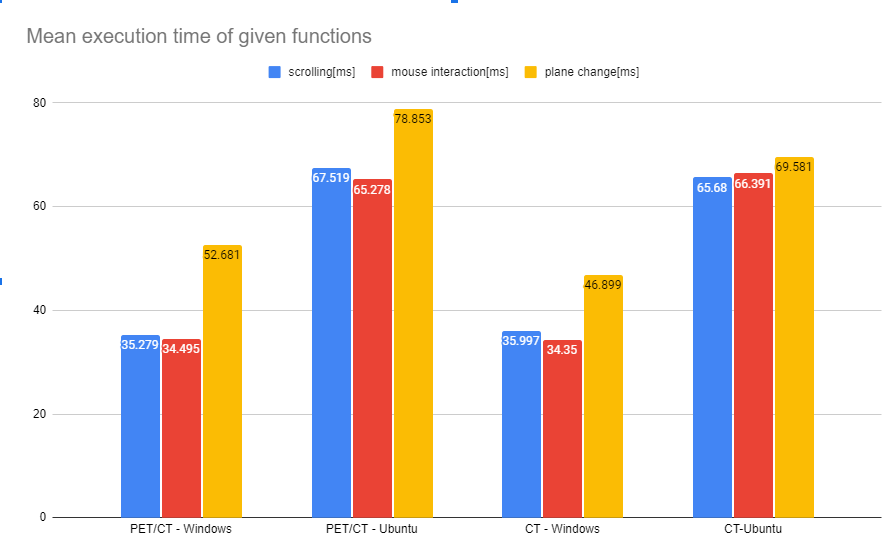
\includegraphics[width=\columnwidth]{Przechwytywanie.png}
	\caption{Execution times depending on function and machine used}
	\label{fig:Przechwytywanie}
	\centering
\end{figure}

Time required for cross section plane change (for example from transverse to sagittal) was defined as a difference in time from invocation of GLFW callback (which itself will be invoked on appropriate user interaction) to end of rendering function execution.
Results of experiments mentioned above are summarized in Figure \ref{fig:Przechwytywanie}. What is clearly visible time required for completion of functions in case of the Ubuntu laptop was longer, yet considering far inferior hardware characteristic it was to be expected, also reduced performance did not affected user experience.


Memory usage was tested using actual data from PET/CT. Data uploaded to display constituted 3 Matricies of Float32, UInt8  and Int16 dataTypes, additionally 2000x8000 matrix holding text data was displayed. 
In case of Windows 10 system Dedicated GPU memory usage was evaluated using Details section of Task Manager and was oscillating between between 38K and 39.5K. In case of Ubuntu Laptop application used to estimate GPU memory usage was Nvidia System Monitor and dedicated GPU memory usage oscillated around 21MB. 

\section{Conclusions}
Medical image segmentation is a complex task requiring knowledge from medicine, engineering and mathematics. In order to make the task of developing such algorithms as manageable as possible multiple software tools were developed. However because of rapid advancements both in machine learning and in medical imaging the need of further tool specialization emerges. Hence although most of the needs of the research community may be met by existing solutions, there are usecases where existing solutions are not adequate for the needs. One of such case are researchers that would like to work in Julia programming language either because of rich ecosystem of scientific libraries or because of high performance both in terms of execution time and development time. In order to be able to develop Medical segmentation algorithms in  Julia programming language one requirement is to be able to complete all the necessary steps using Julia programming language with possible exception of preprocessing which frequently needs to be done only once.

Programming framework presented in this work is the response to changing software enviroment, it is implemented in emerging programming language - Julia. Is implemented with GPU acceleration giving vast performance improvements over CPU based algorithms, and uses modern programming approaches like reactive functional style in GUI programming. Additionally what is critical for convenient rapid prototyping all of the programming process can be done with help of Julia REPL. What is also worth pointing out is a fact that multiple metrics implemented in the presented software are to the best knowledge author are characterized by shortest execution time not only in Julia programming language but among all popular open source solutions. 

In order to make development process even easier in the last chapter author presented additional set of utility functions, that for example adds needed persistency layer  using HDF5 system. Still all of the tools presented in this work are highly composable and may be used in isolation, what constitutes another important advantage of the presented work. 

\section*{Acknowledgement}
The package is open source and available on GitHub https://github.com/jakubMitura14/MedPipe3D.jl under the Apache license. In case of any feature request, bug reporting, contribution propositions contact the author via LinkedIn https://linkedin.com/in/jakub-mitura-7b2013151/ or in the issues section of GitHub repository.

%% If you have bibdatabase file and want bibtex to generate the
%% bibitems, please use
%%
 \bibliographystyle{elsarticle-num} 
 \bibliography{ref}

%% else use the following coding to input the bibitems directly in the
%% TeX file.

% \begin{thebibliography}{00}

% %% \bibitem{label}
% %% Text of bibliographic item

% \bibitem{}

% \end{thebibliography}
\end{document}
\endinput
%%
%% End of file `elsarticle-template-num.tex'.
